% !TEX TS-program = pdflatex
% !TEX encoding = UTF-8 Unicode

% This is a simple template for a LaTeX document using the "article" class.
% See "book", "report", "letter" for other types of document.

\documentclass[11pt, preview]{standalone} % use larger type; default would be 10pt

\usepackage[utf8]{inputenc} % set input encoding (not needed with XeLaTeX)


\usepackage{../../markup}
%%% Examples of Article customizations
% These packages are optional, depending whether you want the features they provide.
% See the LaTeX Companion or other references for full information.

%%% PAGE DIMENSIONS
\usepackage{geometry} % to change the page dimensions
\geometry{a4paper} % or letterpaper (US) or a5paper or....
% \geometry{margin=2in} % for example, change the margins to 2 inches all round
% \geometry{landscape} % set up the page for landscape
%   read geometry.pdf for detailed page layout information

\usepackage{graphicx} % support the \includegraphics command and options
\usepackage{color, tikz}
% \usepackage[parfill]{parskip} % Activate to begin paragraphs with an empty line rather than an indent

%%% PACKAGES
\usepackage{amsmath, amsfonts,amssymb}
\usepackage{booktabs} % for much better looking tables
\usepackage{array} % for better arrays (eg matrices) in maths
\usepackage{paralist} % very flexible & customisable lists (eg. enumerate/itemize, etc.)
\usepackage{verbatim} % adds environment for commenting out blocks of text & for better verbatim
\usepackage{subfig} % make it possible to include more than one captioned figure/table in a single float
\usepackage{tikz}
\usetikzlibrary{arrows}
% These packages are all incorporated in the memoir class to one degree or another...

%%% HEADERS & FOOTERS
\usepackage{fancyhdr} % This should be set AFTER setting up the page geometry
\pagestyle{fancy} % options: empty , plain , fancy
\renewcommand{\headrulewidth}{0pt} % customise the layout...
\lhead{}\chead{}\rhead{}
\lfoot{}\cfoot{\thepage}\rfoot{}

%%% SECTION TITLE APPEARANCE
\usepackage{sectsty}
\allsectionsfont{\sffamily\mdseries\upshape} % (See the fntguide.pdf for font help)
% (This matches ConTeXt defaults)

%%% ToC (table of contents) APPEARANCE
\usepackage[nottoc,notlof,notlot]{tocbibind} % Put the bibliography in the ToC
\usepackage[titles,subfigure]{tocloft} % Alter the style of the Table of Contents
\renewcommand{\cftsecfont}{\rmfamily\mdseries\upshape}
\renewcommand{\cftsecpagefont}{\rmfamily\mdseries\upshape} % No bold!

\newcommand{\N}{\mathbb{N}}
\newcommand{\Prob}{\mathbb{P}}
\newcommand{\Z}{\mathbb{Z}}
\newcommand{\R}{\mathbb{R}}
\newcommand{\Q}{\mathbb{Q}}

\newcommand{\ie}{\textit{i.e.}}
%%% END Article customizations

%%% The "real" document content comes below...

\date{} % Activate to display a given date or no date (if empty),
         % otherwise the current date is printed 

\begin{document}
\config{name}{Probability Spaces and Conditional Probability}
\noindent{\bf Probability Spaces and Conditional Probability}.

\begin{enumerate}
\item Suppose I have a biased coin, with outcomes $H$ and $T$, with the probability of heads $\Prob[H] = \frac{3}{4}$ and the probability of tails $\Prob[T] = \frac{1}{4}$. Suppose I perform an experiment in which I toss the coin 3 times--an outcome of this experiment is $(X_1, X_2, X_3)$, where $X_i \in \{H,T\}$.\\
\begin{enumerate}
\item What is the \textit{sample space} for my experiment?
\begin{Multi}
\begin{enumerate}
\FalseChoice\item $\{H, T\}$
\FalseChoice\item $\{\frac{3}{4}, \frac{1}{4}\}$
\TrueChoice\item $\{(X_1, X_2, X_3) \ s.t. \ X_1, X_2, X_3 \in \{H,T\}\}$
\end{enumerate}
\Hint Review the definition of an sample space in the notes.
\Solution We have three flips, therefore our sample space needs to capture all sequences of length $3$ of possible outcomes.
\end{Multi}
%-----------------------------------------------
\item Which of the following are examples of \textit{events}? Select all that apply.
\begin{Multi}
\begin{enumerate}
\FalseChoice\item $\{(H,H,T), (H,H), (T)\}$
\TrueChoice\item $\{(T, H, H), (H, T, H), (H, H, T), (H, H, H)\}$
\TrueChoice\item $\{(T, T,T)\}$
\TrueChoice\item $\{(T, T, T), (H, H, H)\}$
\TrueChoice\item $\{(T, H, T), (H, H, T)\}$
\end{enumerate}
\Hint Review the definition of an event in the notes.
\Solution Any subset of the sample space is an event. All choices but the first one are valid subsets.
\end{Multi}
%-----------------------------------------------
\item What is the probability of the outcome $H, H, T$? Enter your answer as a fully reduced fraction (i.e. your answer should have the format $x/y$, where $x, y \in \N$ are the smallest possible integers they can be). 
\begin{Freeform}{9/64}
$\Prob[(H,H,T)]$ = 
\Hint Note that the coin tosses are independent, and you know $\Prob[H], \Prob[T]$.
\Solution We need to multiply the probabilities together. We get $\frac{3}{4}\times\frac{3}{4}\times\frac{1}{4}=\frac{9}{64}$.
\end{Freeform}
%-----------------------------------------------
\item What is the probability of the event that my outcome has exactly two heads? Enter your answer as a fully reduced fraction (i.e. your answer should have the format $x/y$, where $x, y \in \N$ are the smallest possible integers they can be). 
\begin{Freeform}{27/64}
$\Prob[$ exactly 2 heads] = 
\Hint Note that the coin tosses are independent, and you know $\Prob[H], \Prob[T]$. How many such outcomes are there, and what is each one's probability? Try a combinatorial approach.
\Solution There are three such outcomes (three places where the single tails can occur). Each such outcome has probability $\frac{9}{64}$ like before. So the total probability is $3\times\frac{9}{64}=\frac{27}{64}$.
\end{Freeform}
\end{enumerate}
\item Consider the drawing of the probability space $S$ below. Here, the blue/purple region is the set of events $B$, the red/purple/orange region is the set of events $R$, and the yellow/orange region is the set of events $Y$. The set of events $P$ is the set of events in both  $B \text{ and } R$, and is represented by the purple region. The set of events $O$ is the set of events in both $R \text{ and } Y$, and is represented by the orange region.

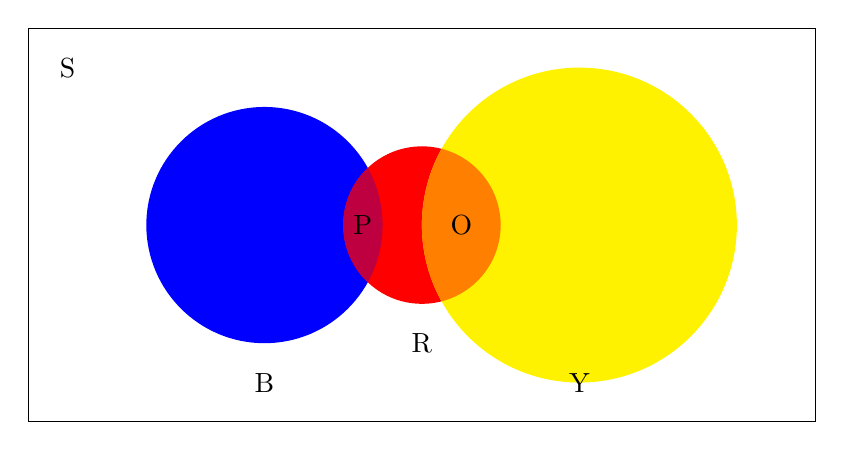
\begin{tikzpicture}[scale=0.5]
  \draw (-10,-5) rectangle (10,5);
  \fill[fill=blue] (-4,0) circle [radius=3];
  \fill[fill=red] (0,0) circle [radius=2];
  \fill[fill=yellow] (4,0) circle [radius=4];
  \begin{scope}
    \clip (0,0) circle [radius=2];
    \fill[fill=purple] (-4,0) circle [radius=3];
    \fill[fill=orange] (4,0) circle [radius=4];
  \end{scope}
  \draw (-9,4) node {S};
  \draw (-4,-4) node {B};
  \draw (0,-3) node {R};
  \draw (4,-4) node {Y};
  \draw (-1.5,0) node {P};
  \draw (1,0) node {O};
\end{tikzpicture}
%\begin{center}
%\includegraphics[width=5cm]{probspace.pdf}
%\end{center}

Assume that we are sampling from $S$ uniformly at random. Please answer the following multiple choice questions about this space, selecting all that apply.
\begin{enumerate}
\item What is $\Prob[R]$, the probability that an element from $S$ is in $R$?
\begin{Multi}
\Hint Recall the definition of probability--the probability of an event $X$ is the number of outcomes for which $X$ occurs divided by the total number of outcomes. 
\begin{enumerate}
\FalseChoice\item $\frac{|R| - |P| - |O|}{|S|}$
\TrueChoice\item $\frac{|R|}{|S|}$
\FalseChoice\item $|R|$
\end{enumerate}
\Solution Since we are sampling uniformly at random, the probabilities are computed by dividing the number of elements in the event of interest ($R$) by the total number of elements ($S$).
\end{Multi}
%-----------------------------------
\item What is $\Prob[R|Y]$, the probability that an element from $S$ is in $R$ given that it is also in $Y$?
\begin{Multi}
\Hint Recall the definition of probability--the probability of an event $X$ is the number of outcomes for which $X$ occurs divided by the total number of outcomes. When we condition on an event $Z$, we are restricting the total outcomes to be outcomes for which $Z$ occurs.
\begin{enumerate}
\FalseChoice \item $\frac{|O|}{|S|}$
\TrueChoice\item $\frac{|O|}{|Y|}$
\TrueChoice\item $\frac{|R \cap Y|}{|Y|}$
\end{enumerate}
\Solution Conditioning on $Y$ is like considering everything outside of $Y$ as not even being there. So we need to restrict $R$ to $Y$ which gives us $Y\cap R=O$. Then we need to divide the number of elements in that region by $|Y|$ which is our new sample space.
\end{Multi}
%-----------------------------------
\item What is $\Prob[R|O]$, the probability that an element from $S$ is in $R$ given that it is in $O$?
\begin{Multi}
\Hint Recall the definition of probability--the probability of an event $X$ is the number of outcomes for which $X$ occurs divided by the total number of outcomes. When we condition on an event $Z$, we are restricting the total outcomes to be outcomes for which $Z$ occurs.
\begin{enumerate}
\TrueChoice \item 1
\TrueChoice \item $\frac{|R \cap O|}{|O|}$
\FalseChoice\item $\frac{|R \cap O|}{|S|}$
\end{enumerate}
\Solution Like before this probability is equal to $\frac{|R\cap O|}{|O|}$. But note that $O\cap R = O$, so this fraction is just $1$.
\end{Multi}
%-----------------------------------
\item What is $\mathbb{P}[P|B]$, the probability that an element from $S$ is in $P$ given it is in $B$?
\begin{Multi}
\Hint Recall the definition of probability--the probability of an event $X$ is the number of outcomes for which $X$ occurs divided by the total number of outcomes. When we condition on an event $Z$, we are restricting the total outcomes to be outcomes for which $Z$ occurs.
\begin{enumerate}
\FalseChoice\item $\frac{|P|}{|S|}$
\TrueChoice\item $\frac{|P|}{|B|}$
\TrueChoice\item $\frac{|B \cap P|}{|B|}$
\end{enumerate}
\Solution Similar to the previous questions, the answer is $\frac{|B\cap P|}{|B|}$. Note that $P\subseteq B$, so $B\cap P=P$.
\end{Multi}
%-----------------------------------
\item What is $\Prob[B \cup R \cup Y]$, the probability that an element of $S$ is in $B$ or $R$ or $Y$?
\begin{Multi}
\Hint Recall the definition of probability--the probability of an event $X$ is the number of outcomes for which $X$ occurs divided by the total number of outcomes. Be careful not to double count!
\begin{enumerate}
\TrueChoice\item $\frac{|B| + |R| + |Y| - |P| - |O|}{|S|}$
\TrueChoice\item $\frac{|B \setminus P| + |R| + |Y\setminus O|}{|S|}$   \hfill ($X \setminus Z = \{ x \ s.t.\ x \in X\text{ and } x \not\in Z\}$)
\FalseChoice\item $\frac{|B| + |R| + |O|}{|S|}$
\end{enumerate}
\Solution We just need to count and make sure that each region inside the union is counted exactly once. This happens in the first two choices. In the last choice, $O$ is counted twice (once from $R$ and once from $O$) as is $P$. So the last choice is not right.
\end{Multi}
%-----------------------------------
\item What is $\Prob[O | R \cup Y]$, the probability that an element of $S$ is in  $O$ given that it is also in $R$ or $Y$?
\begin{Multi}
\Hint Recall the definition of probability--the probability of an event $X$ is the number of outcomes for which $X$ occurs divided by the total number of outcomes. When we condition on an event $Z$, we are restricting the total outcomes to be outcomes for which $Z$ occurs. Be careful not to double count!
\begin{enumerate}
\FalseChoice\item $\frac{|O|}{|S| - |B|}$
\TrueChoice\item $\frac{|O|}{|Y| + |R| - |O|}$
\FalseChoice\item $\frac{|O|}{|Y| + |R|}$
\end{enumerate}
\Solution $O$ is a subset of $R\cup Y$. So in the numerator we just need $|O|$. In the denominator we need $\Prob[R\cup Y]$. Only the second choice gives us that in the denominator.
\end{Multi}
%-----------------------------------
\end{enumerate}
%------------------------------------------------------------------------------------------------------------------------

\item Suppose I have a bag of candy containing 10 chocolate bars, 5 lollipops and 5 toffees. 
\begin{enumerate}
\item If I randomly select a piece of candy to eat, what is the probability that it will be a chocolate bar? Please enter your answer as a decimal. Enter the answer as an exact decimal with a leading zero.
\begin{Freeform}{0.5}
$\Prob[\text{chocolate}]$ = 
\Hint Recall the definition of probability.
\Solution Exactly half of the candies are chocolate bars. So the probability is $1/2$.
\end{Freeform}
%-------------------------------------------
\item Suppose that I am trying to randomly select a candy for a friend who does not like chocolate, so that every time I choose a chocolate I return it to the bag, and I stop when I draw a candy that is not chocolate. What is the probability that I choose a toffee? Enter the answer as an exact decimal with a leading zero.
\begin{Freeform}{0.5}
Probability = 
\Hint Recall the definition of probability--what are we conditioning on?
\Solution Conditioning on the candy not being a chocolate bar, we have a sample space consisting of $5$ lollipops and $5$ toffees. In this space, exactly half of the outcomes are toffees. So the probability is again $1/2$.
\end{Freeform}
%-------------------------------------------
\item Say that I have eaten one chocolate, one toffee, and one lollipop. True or false: now that I have eaten one of each candy, my probability of choosing a chocolate has decreased.
\begin{Choices}
Calculate the probability of drawing a chocolate in the updated bag. 
\begin{itemize}
\FalseChoice\item True
\TrueChoice\item False
\end{itemize}
\Solution In the new space we have $9$ chocolate bars, $4$ toffees and $4$ lollipops. Therefore the new probability of picking a chocolate bar is $9/17$ which is slightly above $1/2$.
\end{Choices}
%-------------------------------------------
\end{enumerate}
%------------------------------------------------------------------------------------------------------------------------
\item {\bf Bayesian Inference.} In this problem, we will work through an example of Bayesian Inference.

Suppose you would like to decide whether to go to on a picnic tomorrow.
You have some data about the weather in the area. You know the following:
\begin{itemize}
\item The probability of rain, $\Prob[R] = 0.2$
\item The probability you see clouds the day before it rains, $\Prob[C|R] = 0.75$
\item The probability you see clouds the day before a clear day, $\Prob[C|\overline{R}] = 0.1$
\end{itemize}
You notice heavy clouds in the sky. If you could calculate the probability that it will rain tomorrow conditioned on the clouds in the sky tonight, then you can make a more informed decision about tomorrow's plans.

You want to calculate $\Prob[R | C]$, the probability that it rains tomorrow if it is cloudy tonight. You remember that by  Bayes' formula, 
\[
\Prob[R|C] = \frac{\Prob[C|R]\Prob[R]}{\Prob[C]}.
\]
You do not know $\Prob[C]$. But, you know that 
\[
\Prob[C] = \Prob[C \cap \overline{R}] + \Prob[C \cap R].
\]
\begin{enumerate}
\item  You can compute $\Prob[C \cap R]$ from the known quantities above. Recall that
\[
\Prob[C \cap R] = \Prob[C|R]\Prob[R]
\] 
What is $\Prob[C \cap R]$? Enter your answer as an exact decimal with a leading zero.
\begin{Freeform}{0.15}
$\Prob[C \cap R]$ = 
\Hint Do you know each of these quantites? Refer to your data above.
\Solution We know that $\Prob[C \cap R] = \Prob[C|R]\Prob[R]=0.75\times 0.2 = 0.15$.
\end{Freeform}
%-------------------------------------------
\item Now, you can compute $\Prob[C \cap \overline{R}]$:
\[
\Prob[C \cap \overline{R}] = \Prob[C|\overline{R}]\Prob[\overline{R}]
\] 
What is  $\Prob[C \cap \overline{R}]$? Enter your answer as an exact decimal with a leading zero.
\begin{Freeform}{0.08}
$\Prob[C \cap \overline{R}]$ = 
\Hint Do you know each of these quantites? Refer to your data above.
\Solution We have $\Prob[C\cap \overline{R}] = \Prob[C|\overline{R}]\Prob[\overline{R}]=0.1\times (1-0.2)=0.08$.
\end{Freeform}
%-----------------------------------
\item Finally, calculate $\Prob[R|C] = \frac{\Prob[C|R]\Prob[R]}{\Prob[C \cap \overline{R}] + \Prob[C \cap R]}$. Enter your answer as a decimal with a leading 0 and 2 decimal place's percision (i.e. $0.xy$ where $x,y$ are digits). 
\begin{Freeform}{0.65}
$\Prob[R|C]$ = 
\Hint Refer to your Bayes' formula above, and plug in your known quantities. 
\Solution We have calculated the numerator already. It is $0.15$. The denominator is the sum of two terms, each of which has already been computed. So the denominator is $0.15+0.08=0.23$. Therefore the probability $\Prob[R|C]$ is simply $0.15/0.23\simeq 0.65$.
\end{Freeform}
%-----------------------------------
\item Your prior was $\Prob[R]$, the probability that it rains tomorrow. Assuming you do not want to get rained on, will you be more or less likely to go on a picnic tomorrow considering your posterior probability $\Prob[R|C]$? 
\begin{Choices}
Is the posterior probability that it will rain greater than $0.5$? Was the prior probability greater than $0.5$?
\begin{itemize}
\FalseChoice\item More
\TrueChoice\item Less
\end{itemize}
\Solution Since the posterior is greater, it will be more likely to rain tomorrow, and therefore we should be less likely to go on a picnic.
\end{Choices}
%-----------------------------------
\end{enumerate}
\item {\bf Which is the biased coin?} In this problem, we will use Bayesian 
inference to try and distinguish a biased coin from a fair coin.

Suppose I have 2 coins. Let's call them $A$ and $B$. Coin $A$ is
unbiased,~\ie,~when you flip it, it comes up with a heads with probability
exactly $0.5$, or about half the time. Coin $B$ is biased. When you flip it, it
comes up with a heads with probablility $0.75$, or about three fourths of the
time.

The problem is that outwardly, the two coins are identical and
indistinguishable. I can't tell which is which just by looking at them, or
weighing them, or subjecting them to any physical test. All I can do is flip the
coins many times, and hope to tell them apart based on the outcomes of these
flips.

\begin{enumerate}
%-------------------------------------------
\item{So I pick up one of these coins at random and flip it a $100$ times, and I get 
    $50$ heads.}
\begin{Choices} 
Given the outcome above, what is the probability that the coin I picked is 
unbiased?
\begin{itemize}
\FalseChoice\item 0.0
\FalseChoice\item 0.5
\FalseChoice\item 1.0
\TrueChoice\item $\frac{1}{1 + \left(\frac{3}{4}\right)^{50}}$
\FalseChoice\item $\frac{1}{1 + \left(\frac{1}{2}\right)^{100}}$
\FalseChoice\item $\frac{\dbinom{100}{50}\frac{1}{2^{100}}}{\dbinom{100}{75} \left(\frac{3}{4}\right)^{100} + \dbinom{100}{50} \left(\frac{1}{2}\right)^{100}}$
%\FalseChoice\item $\frac{\left(\frac{3}{4}\right)^{25}}{\left(\frac{3}{4}\right)^{25} + \left(\frac{1}{4}\right)^{25}}$
\FalseChoice\item $\frac{1}{1+\left(\frac{1}{3}\right)^{25}}$
\end{itemize}
\Solution Let $A$ be the event that I get $50$ flips out of the $100$, and let $B$ be the event that I pick the unbiased coin. Then $\Prob[B]=0.5$. We also have $\Prob[A|B]=\binom{100}{50}(1/2)^{100}$, since there are $\binom{100}{50}$ ways to pick the $50$ heads and each such configuration happens with probability $(1/2)^{100}$.

We also have $\Prob[A|\overline{B}]=\binom{100}{50}(3/4)^{50}(1/4)^{50}$ since if we pick the biased coin, there are again $\binom{100}{50}$ configurations with $50$ heads and each occurs with probability $(3/4)^{50}(1/4)^{50}$.

Now using the Bayes' formula we have
$$\Prob[B|A] = \frac{\Prob[A|B]\Prob[B]}{\Prob[A|B]\Prob[B]+\Prob [A| \overline{B}]\Prob[\overline{B}]} =
\frac{\Prob[A|B]\times 0.5}{\Prob[A|B]\times 0.5 + \Prob[A|\overline{B}]\times 0.5}$$

And the last part is equal to
$$\frac{(1/2)^{100}}{(1/2)^{100}+(3/4)^{50}(1/4)^{50}}$$
which can be further simplified into $\frac{1}{1+(3/4)^{50}}$.
\end{Choices}
%-------------------------------------------
\item{Now I pick up the other coin and flip \textit{it} a $100$ times, 
    and I get $75$ heads.}
\begin{Choices} 
    Given the two outcomes above (\ie,~the heads counts from both sets of $100$ 
    flips), what is the probability that the first coin that I picked is 
    unbiased?
\begin{itemize}
\FalseChoice\item 0.0
\FalseChoice\item 0.5
\FalseChoice\item 1.0
\FalseChoice\item $\frac{1}{1 + \left(\frac{3}{4}\right)^{50}}$
\FalseChoice\item $\frac{1}{1 + \left(\frac{1}{2}\right)^{100}}$
\FalseChoice\item $\frac{\dbinom{100}{50}\frac{1}{2^{100}}}{\dbinom{100}{75} \left(\frac{3}{4}\right)^{100} + \dbinom{100}{50} \left(\frac{1}{2}\right)^{100}}$
%\TrueChoice\item $\frac{\left(\frac{3}{4}\right)^{25}}{\left(\frac{3}{4}\right)^{25} + \left(\frac{1}{4}\right)^{25}}$
\TrueChoice\item $\frac{1}{1+\left(\frac{1}{3}\right)^{25}}$
\end{itemize}
\Solution Same as before, we just need to use the Bayes' formula. If $C$ is the event of seeing 75 heads for the second coin, then $\Prob[C|\overline{B}] = \binom{100}{75}(1/2)^{100}$ and $\Prob[C|B]=\binom{100}{75}(3/4)^{75}(1/4)^{25}$.

Note that $A$ and $C$ are independent conditioned on $B$, meaning that once we fix whether we picked the biased coin or the unbiased coin, the two events $A$ and $C$ become independent (since they involve two series of unrelated coin tosses). So we have $\Prob[A\cap C|B]=\Prob[A|B]\Prob[C|B]$ and similarly $\Prob[A\cap C|\overline{B}]=\Prob[A|\overline{B}]\Prob[C|\overline{B}]$. We need $\Prob[B|A\cap C]$. We can again use the Bayes' formula and we end up with

$$\Prob[B|A\cap C] = \frac{(1/2)^{100}\times (3/4)^{75}(1/4)^{25}}{(1/2)^{100}\times (3/4)^{75}(1/4)^{25} + (3/4)^{50}(1/4)^{50}\times (1/2)^{100}}$$

This further simplifies into $\frac{1}{1+(1/3)^{25}}$.

\end{Choices}
%-----------------------------------
\end{enumerate}
%-----------------------------------

\item {\bf Accounting fraud. }There are $3$ ways a CEO can 
    commit accounting fraud:~(a)~he can overstate revenue by booking fake 
    orders,~(b)~he can overstate profits by recording near-term expenses as 
    long-term capital expenses, and~(c)~he can understate liabilities by making 
    overly optimistic assumptions about the growth prospects of the company's 
    pension funds. In the United States, $50\%$ of CEOs commit fraud~(a), $20\%$ 
    of CEOs commit fraud~(b), $15\%$ of CEOs commit both fraud~(a) and 
    fraud~(b), and all CEOs commit fraud~(c).
    
    The probability of getting caught if a CEO does~(a) is $0.01$, independent 
    of whether or not he commits other kinds of fraud. Similarly, the 
    probability of getting caught if he does~(b) is $0.05$, and of getting 
    caught if he does~(c) is $0.001$.
    
\begin{enumerate}
%-------------------------------------------
    \item{What are the chances (rounded to 2 decimal places) that a CEO who 
            perpetrates all $3$ kinds of fraud will get caught?}
\begin{Choices}
\begin{itemize}
\FalseChoice\item 0.21
\FalseChoice\item 0.76
\TrueChoice\item 0.06
\FalseChoice\item 0.01
\FalseChoice\item 0.00
\end{itemize}
\Solution If $A, B, C$ are the events of getting caught for each of the three frauds, then we are interested in $\Prob[A\cup B\cup C]$. But note that this is simply $1-\Prob[\overline{A}\cap \overline{B}\cap \overline{C}]$. Since $\overline{A}, \overline{B}, \overline{C}$ are independent, we have $\Prob[\overline{A}\cap \overline{B}\cap \overline{C}]=(1-0.01)(1-0.05)(1-0.001)\simeq 0.94$. Therefore $\Prob[A\cup B\cup C]\simeq 0.06$.
\end{Choices}
%-------------------------------------------
\item{You read on the front page of the Wall Street Journal that the CEO of 
    TrustMe, Inc. (for all practical purposes, a randomly chosen CEO) has been 
    arrested for accounting fraud. What are the chances (rounded to $2$ decimal 
    places) that this CEO perpetrated at least $2$ kinds of fraud?}
\begin{Choices}
\begin{itemize}
\FalseChoice\item 0.00
\FalseChoice\item 0.95
\FalseChoice\item 1.00
\FalseChoice\item 0.33
\TrueChoice\item 0.97
\end{itemize}
\Solution We can partition the sample space into $4$ parts. Let's call the CEOs who perpetrate all frauds $D$, the ones who perpetrate only type (a) and (c) as $E$, the ones who perpetrate only type (b) and (c) as $F$, and the ones who perpetrate only type (c) as $G$. Also let $A, B, C$ be the events of being arrested for frauds of type (a), (b), (c) respectively. Then we are interested in $\Prob[D\cup E\cup F|A\cup B\cup C]$. To use the Bayes' formula we need compute $\Prob[A\cup B\cup C|x]\Prob[x]$ where $x$ ranges over $D, E, F, G$.

We have $\Prob[A\cup B\cup C|D] = (1-(1-0.01)(1-0.05)(1-0.001))$ and $\Prob[D]=0.15$. Therefore $\Prob[A\cup B\cup C|D]\Prob[D]\simeq 0.009$.

We have $\Prob[A\cup B\cup C|E] = (1-(1-0.01)(1-0.001))$ and $\Prob[E]=0.5-0.15=0.35$. Therefore $\Prob[A\cup B\cup C|E]\Prob[E]\simeq 0.00385$.

We have $\Prob[A\cup B\cup C|F] = (1-(1-0.05)(1-0.001))$ and $\Prob[F]=0.2-0.15=0.05$. Therefore $\Prob[A\cup B\cup C|F]\Prob[F]\simeq 0.00255$.

We have $\Prob[A\cup B\cup C|G] = 0.001$ and $\Prob[G] = 1-\Prob[D]-\Prob[E]-\Prob[F]=0.45$. Therfore $\Prob[A\cup B\cup C|G]\Prob[G] = 0.00045$.

Now using the Bayes' formula we get

$$\Prob[D\cup E\cup F|A\cup B\cup C] = \frac{0.009+0.00385+0.00255}{0.009+0.00385+0.00255+0.00045} \simeq 0.97.$$

So the chances are roughly 97\%.
\end{Choices}
%-------------------------------------------
\item{What are the chances (rounded to $2$ decimal 
    places) that the above CEO perpetrated exactly $2$ kinds of fraud?}
\begin{Choices}
\begin{itemize}
\TrueChoice\item 0.40
\FalseChoice\item 0.60
\FalseChoice\item 0.20
\FalseChoice\item 0.10
\FalseChoice\item 1.00
\end{itemize}
\Solution This time we are interested in $\Prob[E\cup F|A\cup B\cup C]$. We can reuse the computations from last time and the Bayes' formula to get

$$\Prob[E\cup F|A\cup B\cup C]=\frac{0.00385+0.00255}{0.009+0.00385+0.00255+0.00045}\simeq 0.40.$$

So the chances are roughly 40\%.
\end{Choices}
%-----------------------------------
\end{enumerate}
%-----------------------------------

\end{enumerate}

%--------------------------------------------------------------------------------------------------------------------------
\end{document}
